% =============================================================================
% Template dissertation using the qdissertation class
% =============================================================================
% This file is the main entry point. Build: make (uses latexmk; see Makefile).
% Default engine: lualatex. To use another: make ENGINE=pdf or make ENGINE=xe.
%
% SPDX-FileCopyrightText: 2026 Frank Langbein <frank@langbein.org>
% SPDX-License-Identifier: LPPL-1.3c
% SPDX-License-Identifier: CC-BY-SA-4.0
%
% This template and other .tex/.bib files in this directory are part of the
% same work and may be distributed and/or modified under the LaTeX Project
% Public License (LPPL), version 1.3c. See LICENSE file.
%
% -----------------------------------------------------------------------------
% Overview (qdissertation class)
% -----------------------------------------------------------------------------
% The class is a wrapper around the standard book class. Layout: A4, 12pt,
% 3cm margins; single line spacing; ragged-right; main text 12pt, footnotes and
% captions at least 11pt; preliminary pages in roman numerals, then Arabic
% for main matter. Chapter style: top bar in header, ``Chapter N'' or
% ``Appendix A'' in header; number/letter and title on first line of chapter.
%
% -----------------------------------------------------------------------------
% Report structure
% -----------------------------------------------------------------------------
% Main body: Introduction, Background, Methodology (or ``Specification, Design
% and Implementation'' / ``Approach''), Results and Evaluation, Conclusions and
% Future Work, Reflection on Learning. Chapter~3 can be adapted or split; not all
% sections apply to every project (system design, research, AI/ML). See each
% chapter file for details and alternatives.
%
% Suggested sections at a glance (omit/rename as needed):
%   1 Introduction:    Motivation and context; Aims and objectives; Contributions;
%                      Dissertation structure. Optional: Scope, Terminology.
%   2 Background:      Context; Related work (or Literature review); Problem statement.
%                      Optional: Theory and concepts; Stakeholders and constraints.
%   3 Methodology:     Depends on project type. System design: Specification, System
%                      design, Implementation. Research: Research design, Literature
%                      and evidence, Approach and solution, Implementation. AI/ML:
%                      Specification, Datasets, AI/ML models, System design, Implementation.
%                      Optional: Ethical considerations; Summary.
%   4 Results:         Setup (or Experimental setup); Results; Discussion; Limitations.
%                      Optional: Ablation studies; Comparison with baselines.
%   5 Conclusions:     Conclusions; Future work.
%   6 Reflection:      Critical narrative; Analysis and application; Implications
%                      for future practice. (Omit chapter if not required.)
%
% -----------------------------------------------------------------------------
% Variations (degree, structure)
% -----------------------------------------------------------------------------
% Select your degree via \degree below; commented alternatives shown for
% BSc, MSc.
%
% -----------------------------------------------------------------------------
% Class options
% -----------------------------------------------------------------------------
% Font: sans (default), serif, or hacker;
%   serif = serif text and math; hacker = typewriter/monospace open-source font throughout.
% Layout: oneside (default) or twoside.
% Citation: numeric (default) = plainnat, [1], [1,2]; harvard = agsm, (Author, 2000).
% Alignment: raggedright (default) = ragged-right; justified = fully justified text.
% Line spacing: single (default); onehalfspacing; or linespread115/linespread12
%   for institutions allowing 1.0--1.3.
% Paragraph style: parskip (default) = space between paragraphs, no first-line indent;
%   parindent = traditional first-line indent, minimal parskip.
% Optional typography:
%   fullwidth  = enable \begin{fullwidth}...\end{fullwidth} and fullwidthfigure/
%                fullwidthtable environments that extend into the margin (requires
%                changepage or chngpage).
%   italic = chapter, section, subsection and captions in italic (default: bold/roman).
% Engine: pdfTeX vs XeLaTeX/LuaLaTeX is detected for font setup.
%
% Defaults (no option): link colour DarkBlue, cite/URL colour DarkGreen; tight list
% margins; quote, quotation, and verse in smaller type with indents;
% \epigraph{quote}{source} for chapter/section-opening quotes.
% See Section~\ref{sec:ch1-reference} in Chapter~1 for examples of \newthought,
% fullwidth, fullwidthfigure, quote, and epigraph.
%
% -----------------------------------------------------------------------------
% Metadata and title page
% -----------------------------------------------------------------------------
% \title, \author, \degree, \university, \date drive the generated title page.
%
% -----------------------------------------------------------------------------
% License and copyright (SPDX)
% -----------------------------------------------------------------------------
% \copyrightholder defaults to \author; \licenseyear defaults to current year.
% When \license is set: (1) a copyright page is inserted after the abstract;
% (2) a License chapter is inserted just before the bibliography.
% If qdissertation-licenses.tex is present, the class loads it for full
% license text; otherwise name + URL only.
%
% -----------------------------------------------------------------------------
% Float placement (figures, tables, algorithms)
% -----------------------------------------------------------------------------
% Placement letters: h = here, t = top, b = bottom, p = float page. E.g.\@
% [htbp], [t], [!t]. Use [H] (float pkg) sparingly. The class relaxes float
% parameters so more floats fit per page.
%
% -----------------------------------------------------------------------------
% Headings: use title case for chapter titles (capitalise major words; keep
% articles, conjunctions, and short prepositions lowercase unless first/last
% word). Use sentence case for sections, subsections, and below (only the
% first letter and proper nouns capitalised). Or adjust as preferred, but keep
% it consistent.
%
% -----------------------------------------------------------------------------
% LaTeX formatting: \citep/\citet (not \cite); ~ before \citep/\citet after a word;
% \@ after abbreviation; ~ for non-breaking (Fig.~1); -- en-dash, --- em-dash.
%
% -----------------------------------------------------------------------------
% Reviewer comments: %ID (e.g.\@ %F) at line start, space after ID. Include
% comments directly in the text and discussions or questions can be included
% as comments afterwards. Generally, these comments should be inserted closely
% after the sentence or element it refers to. Delete the comments when
% addressed; do not keep ``for checking''. Edits can be easier found via git
% diffs. Find comments with: grep -r '^%[A-Za-z] ' *.tex */*.tex
%
% -----------------------------------------------------------------------------
% Footnotes: prefer putting short asides in parentheses in the main text. Use
% footnotes only sparingly when they add value (e.g.\@ translations, optional
% clarifications that would interrupt the flow).
%
% -----------------------------------------------------------------------------
% Word count: run ``make wordcount'' (texcount -inc; per-file and total with
% caption words shown separately so you can apply your institution's rules).
% Word limits typically apply to main body only; exclude front matter, captions,
% appendices. Confirm your institution's word limits and structure before submission.
%
% -----------------------------------------------------------------------------
% Submission: ensure PDF has embedded fonts (pdflatex does this by default),
% and is compatible with your institution's requirements (e.g. no encryption, be
% careful with obfuscation).
% =============================================================================
\documentclass[sans,oneside,numeric,raggedright,fullwidth]{qdissertation}

% -----------------------------------------------------------------------------
% Optional: use a different acronyms file
% -----------------------------------------------------------------------------
% \renewcommand{\qdissertationacronymfile}{my-acronyms.tex}

% -----------------------------------------------------------------------------
% Useful packages for dissertation writing
% -----------------------------------------------------------------------------

% Tables
\usepackage{tabularray}      % Flexible column types, rules, longtblr for multi-page tables
\usepackage{booktabs}        % Alternative (traditional): \toprule, \midrule, \bottomrule
\usepackage{longtable}       % Tables that span multiple pages (or use tabularray longtblr)
%\usepackage{multirow}        % Span multiple rows in tables
%\usepackage{multicol}        % Multiple columns in text/tables
%\usepackage{colortbl}        % Coloured rows/cells in tables

% Math, symbols, related
\usepackage{mathtools}       % Extensions to amsmath (matrix envs, \DeclarePairedDelimiter)
\usepackage{pifont}          % Dingbat symbols, e.g. \ding{51}, \ding{43}
\usepackage{siunitx}         % Units and numbers: \SI{3}{m/s}, \num{1000}
\usepackage{relsize}         % \textlarger, \textsmaller for relative font sizing
\usepackage[version=4]{mhchem} % Chemical formulae: \ce{H2O}, \ce{CO2}, \ce{^1H-NMR}

% Floats
\usepackage{float}           % [H] = here definitely
\usepackage{stfloats}        % Improved placement for bottom floats
\usepackage{subcaption}      % Subfigures with (a), (b) and per-subfigure captions
\usepackage{rotating}        % \begin{sidewaystable}, \begin{sidewaysfigure} for wide content

% Algorithms
\usepackage{algorithm}       % Numbered algorithm floats and List of Algorithms
\usepackage[noend]{algpseudocode}

% Other useful packages
% \usepackage{lipsum}          % Placeholder text: \lipsum[n], \lipsum[1-5], etc.
\usepackage{enumitem}        % Customise list labels, spacing
\usepackage{verbatim}        % \begin{verbatim} ... \end{verbatim} for code
\usepackage{afterpage}       % \afterpage{\clearpage} to clear after current page

% -----------------------------------------------------------------------------
% Dissertation metadata
% -----------------------------------------------------------------------------
\title{Solving Solitaire Battleships Using Integer Linear Programming}
\author{Morgan Diment}
% Degree
\degree{BSc Computer Science}
% \degree{MSc Advanced Computer Science}
\university{Cardiff University}
\date{May 2026}

% License and copyright following SPDX. (optional; comment out if not needed).
% Needs qdissertation-licenses.tex for license text in the License chapter.
% \license{CC-BY-SA-4.0}
% \copyrightholder{Morgan Diment}
% \licenseyear{2026}

\begin{document}

\frontmatter

% \maketitle{...} produces: title page, (copyright page if \license set), abstract,
% then frontlists: TOC, List of Figures, List of Tables, List of Algorithms,
% List of Acronyms (if acronyms.tex defines \newacronym).
% Add \dedication{...} and \makededication separately if desired.
\maketitle{%
  % Abstract: typically 200--300 words. State problem, methods, and main results.
  Battleship Solitaire is a deterministic logic puzzle, with its decision problem being NP-Complete. This makes a suitable testbed for advanced combinatorial optimisation techniques.
  This dissertation compares two Integer Linear Programming (ILP) puzzle formulations that were originally proposed by Meuffels and den Hertog, and quantifies their behaviour under exponential scaling.
  A Cell-based model represents the grid as a state matrix per individual cell, using shape-transition and adjacency constraints.
  A Ship-based model uses candidate generation to find valid ship placements and resolves geometric conflicts with Edge-Based Set Packing. 
  A third variant adds four classes of valid inequalities to the Cell model, to study polyhedral tightening.
  
  To benchmark these formulations, an automated framework was developed using Python and Gurobi. A \gls{csplib} Prolog parser, a procedural puzzle generator that produces feasible instances on grids up to $30 \times 30$, and a thread-safe CustomTkinter interface for interactive solving were engineered.
  Across 150 generated instances and the standard $10 \times 10$ \gls{csplib} dataset, the results show the Ship model dominates, solving $30 \times 30$ zero-hint instances in under \SI{2}{\second}. The Cell model required up to \SI{23}{\second} for the same configurations. 
  Branch-and-Bound node counts remained near unity for all models, isolating the Cell-model's bottleneck to matrix density rather than search-tree depth.
  A constraint ablation study further showed that valid inequalities are scale-dependent. At 900 cells, they reduce the solve time by approximately \SI{1.3}{\second}, but introduce overhead at smaller scales.
  The findings re-frame ILP performance for spatial logic problems as a question of matrix sparsity and root-node relaxation, not search-tree pruning.
}

% -----------------------------------------------------------------------------
% Optional front-matter chapters (unnumbered)
% -----------------------------------------------------------------------------

% Replace with your dedication (one or two lines); optional.
% \dedication{%
%   To my family.%
% }

\chapter{Acknowledgements}\label{chap:acknowledgements}
% Replace with your acknowledgements. Here you can also acknowledge any contributions from other
% parties to the work.
I would like to thank my supervisor Jandson Santos Ribeiro Santos for his academic support throughout the project. Your insight and knowledge helped me stay on the right path with this work.

I would also like to thank my close ones who have supported me during this project. The behind-the-scenes help did more than you'll ever know. 

%\chapter{Declaration}
% Replace with your declaration (e.g. that the work is your own, and any
% required statements on collaboration, publications, or word count).
% Often this is submitted in separate forms or not needed, and does not
% have to be here.
%This dissertation is the result of my own work. Where reference is made to other work, this is indicated in the text.

%\chapter{Publications, data and code}
\chapter{Data and Code}\label{chap:datacode}
% List publications, if available or maybe planned, and state where data and code produced for this
% dissertation are available. Note, you usually must submit any sources and similar you have
% written with your dissertation.
% Replace with your own entries; you can use \citep{key} for publications.

%\section{Publications}
% Papers (and optionally other outputs) that form part of or arise from this thesis.
% These can also be discussed in the introduction (what has been published or is planned).
%\begin{enumerate}
%  \item Author. Title. \textit{Journal}, volume, pages, year.~\citep{example-paper}
%\end{enumerate}

\section{Data}\label{sec:data}
% Datasets produced in this work and where they are available (repository, DOI, or ``on request'').
The standard datasets utilised for the baseline validation were sourced from the Constraint Satisfaction Problem Library meuffels-battleship\citep{csplib:prob014}. The specific Solitaire Battleship (Problem 014) data is available at: \url{https://www.csplib.org/Problems/prob014/data/}.

\section{Code}\label{sec:code}
% Software or code produced in this work and where it is available (repository, DOI, etc.).
Code produced for this dissertation is available from: \url{https://github.com/morgandiment/Battleship-ILP}.

The LaTeX full report is available at: \url{https://github.com/morgandiment/dissertation-report}.

Gurobi \citep{gurobi2024} was used under the Academic Named User License. More information is available at: \url{https://www.gurobi.com/academics}. 

\chapter{Declaration of AI Usage}\label{chap:ai-declaration}

In accordance with the CM3203 project guidelines, I declare the use of two AI assistive technologies during this project. Each was used in a supporting capacity. Neither was used to author the project's mathematical, architectural or analytical content.

Google's Gemini Large Language Model \citep{gemini} was involved in three instances:
\begin{itemize}
  \item \textbf{Diagnostic Assistance:} When the CustomTkinter \gls{gui} began crashing with \verb|NSInternalInconsistencyException| under macOS, Gemini was consulted to identify the underlying cause as a main-thread / background-thread boundary violation in AppKit. The solution (a thread-safe \verb|TextboxRedirector| dispatching through \verb|tkinter.after()|) was then derived independently and is the implementation reproduced in Section~\ref{subsec:platform-challenges-thread-safety}.
  \item \textbf{Boilerplate Regex Syntax:} The \gls{csplib} Prolog parser uses a single \verb|re.compile| call (Section~\ref{subsec:data-structures-parsing}). Gemini provided the initial \verb|\s*\(\s*(\d+)\s*,| escape pattern; the five capture groups, the \verb|re.DOTALL| flag, and the secondary hint-extraction regex were authored manually after testing the pattern against \verb|data/csplib.pl|.
  \item \textbf{LaTeX Typesetting of Derived Equations:} Several constraint equations in Sections \ref{sec:math-formulation-cell}--\ref{sec:valid_inequalities} were derived by hand from Meuffels~\citep{meuffels-battleship} and from analysis of the implemented Gurobi constraints, then typeset in LaTeX with Gemini's syntax assistance for the alignment and subscript notation. The mathematical content of every equation is original work. Gemini's contribution was limited to the surrounding markup.
\end{itemize}

Anthropic Claude~\citep{claude} was used during the report-writing phase as a structured reviewer and consistency checker. Specifically:
\begin{itemize}
  \item \textbf{Code--report consistency review:} Claude was given access to the source code for the implementation and report, and was asked to identify inconsistencies between the two. These inconsistencies found were then re-written in the report by myself, or modified in the code to match the behaviour previously reported.
  \item \textbf{Editorial review:} Claude flagged residual typos, grammatical errors, weak phrasing, and figure caption thinness across the chapters. Each flagged change was reviewed and either accepted in modified form or rejected. Suggestions were not pasted in full.
  \item \textbf{Build pipeline diagnosis:} The List of Acronyms was failing to render in the compiled PDF. Claude identified the missing \verb|makeglossaries| step in the LaTeX Workshop build to fix it.
\end{itemize}

The system architecture (Section~\ref{sec:system-architecture}), the formal mathematical specifications of both \gls{ilp} models (Sections~\ref{sec:math-formulation-cell} and~\ref{sec:math-formulation-ship}), the four valid inequalities (Section~\ref{sec:valid_inequalities}), the procedural puzzle generator (Section~\ref{subsec:procedural-puzzle-gen-algo}), the evaluation methodology and findings (Chapter~\ref{ch4}), the conclusions and future work (Chapter~\ref{ch5}), and the reflection (Chapter~\ref{ch6}) were authored by myself, with the AI tools used only as described above.

To mitigate the risk of hallucinated output from either tool, every AI suggestion was reviewed before integration, and tested for behavioural correctness against the unit tests in \verb|tests/| (which validate both ILP formulations against feasibility-checked reference instances via \verb|BattleshipBoard.is_valid_solution|), and cross-checked against Meuffels~\citep{meuffels-battleship} (for mathematical content). No suggestion was incorporated unmodified.

\mainmatter

% -----------------------------------------------------------------------------
% Main chapters (suggested structure in each chapter file; adjust to your project)
% -----------------------------------------------------------------------------
\chapter{Introduction}\label{ch1}
% =============================================================================
% CHAPTER 1: Introduction
% =============================================================================
% SPDX-FileCopyrightText: 2026 Frank Langbein <frank@langbein.org>
% SPDX-License-Identifier: LPPL-1.3c
%
% Suggested sections: Motivation and context; Aims and objectives; Contributions;
% Dissertation structure (roadmap). Optional: Scope (boundaries of the work),
% Terminology or key terms. Start with a short chapter intro (no \section) before
% the first section. This file also demonstrates template features; see
% Section~\ref{sec:ch1-reference}. Remove that section for your own report.
% =============================================================================

% -----------------------------------------------------------------------------
% Chapter intro (no section): one short paragraph before the first \section
% -----------------------------------------------------------------------------
% This chapter introduces the dissertation. It outlines the motivation and context for the work, the aims and objectives, the main contributions, and the structure of the remaining chapters. The following sections expand on each of these.

% -----------------------------------------------------------------------------
% Motivation and context (typical first section)
% -----------------------------------------------------------------------------
% Use \section, \subsection, \label{key}. Refer with \ref{key} or \autoref{key}.

\section{Motivation and Context}\label{sec:motivation}

This dissertation focusses on the game of Battleship Solitaire, not to be confused with the more commonly known two-player Battleship game. The solitaire version is a deterministic, logic-based puzzle game played by a single person. The aim is to reconstruct a solution on the grid using the given row/column tallies, and individual cell hints.

This is an NP-complete problem, which is the main motivation factor behind this project. As the grid size increases or the number of hints provided decreases, the search space explodes combinatorially.

Because it is NP-complete, brute-force guessing is mathematically infeasible for large boards. Therefore, the problem serves as ideal testbed for advanced optimisation techniques, such as \gls{ilp}, combined with modern-day constraint satisfaction solvers.

Existing literature proposes multiple ways to translate the rules of Solitaire Battleship into linear algebra. One method uses modelling based on the cells, one models based on the ships. The comparison of these sets the stage for this project. 

% \newthought{This template illustrates} the structure and style of a dissertation using the Qyber dissertation class. As in a real introduction, you would state the problem domain, why it matters, and how your work fits. Acronyms use the long-short style: first use gives the full form (e.g.\@ \gls{uk}); later use \acrshort{api} or \acrlong{api} when you need only short or long.

% As shown in previous work~\citep{example-paper}, we follow standard practice.
% %F Clarify whether this applies to all cases.
% \citet{example-book} provide a longer treatment; multiple citations: \citep{example-paper,example-conf}. You can link to other chapters (e.g.\@ Chapter~\ref{ch2}, Section~\ref{sec:objectives}) and to figures (Fig.~\ref{fig:demo}). The class provides \url{https://example.com} and \href{https://example.com}{link text} for URLs and hyperlinks.

% -----------------------------------------------------------------------------
% Aims and objectives (typical second section)
% -----------------------------------------------------------------------------
% Use \citep{} (parenthetical) or \citet{} (narrative), not \cite.

\section{Aims and Objectives}\label{sec:objectives}

The main aim of the project is to determine the most computationally efficient \gls{ilp} paradigm for solving the NP-Complete Battleship Solitaire problem through comparative analysis of two \gls{ilp} formulations, with one additional variant.

To achieve this aim successfully, the project will have the following objectives:

\begin{enumerate}[label=\textbf{O\arabic*:}, leftmargin=*]
  \item To define and implement two \gls{ilp} formulations for the Battleship ruleset. The first being a Cell-based (Big-M) constraint model, and the second a Ship-based (Set Packing) candidate model.
  \item To engineer a scalable, automated evaluation environment that integrates a puzzle generator, a standard \gls{csplib} format parser, and the Gurobi optimisation engine to facilitate standardised solver benchmarking.
  \item To construct a decoupled \gls{gui}, built on a layered architecture with thread-safe message passing between a Gurobi background solver and the CustomTkinter front-end, allowing for the real-time visualisation of solver outputs and the interactive construction of problems.
  \item To conduct a systematic evaluation comparing the computational overhead, search-tree pruning efficiency, and scalability limits of the formulated \gls{ilp} encodings against datasets of varying heuristic difficulty and grid dimensions. 
\end{enumerate}

% -----------------------------------------------------------------------------
% Contributions (typical third section)
% -----------------------------------------------------------------------------

\section{Contributions}\label{sec:contributions}

This dissertation presents a comprehensive algorithmic analysis of \gls{ilp} applied to Battleship Solitaire, an NP-Complete problem. The main contributions of this research are:

\begin{itemize}
  \item \textbf{Automated Evaluation Pipeline and Generator:} The development of a robust Python framework capable of parsing standard \gls{csplib} Prolog datasets, alongside a dynamic puzzle generator designed to create mathematically valid instances up to $30 \times 30$ in size for scalability analysis.
  \item \textbf{Comparative \gls{ilp} Formulations:} The formal mathematical specification and Gurobi implementation of two distinct solver paradigms: a Cell-based model utilizing Big-M boundary constraints, and a Ship-based model employing candidate generation and Edge-Based Set Packing.
  \item \textbf{Constraint Impact Analysis and Tuning:} A Constraint Impact Analysis revealed the 'Overhead vs. Pruning' trade-off, demonstrating that while explicit tally logic reduced solve times on hard instances by pruning dead-end search branches, redundant parity constraints introduced matrix bloat affected performance in certain conditions.
  \item \textbf{Scalability and Performance Discovery:} Conclusive evidence demonstrating that the Ship-based Set Packing formulation strictly dominates the Cell-based approach. The Ship model maintains an immense speed advantage, efficiently solving $30 \times 30$ zero-hint instances in under \SI{2}{\second}, where the Cell model severely weakens, taking an average of \textasciitilde\SI{11}{\second}.
\end{itemize}

% -----------------------------------------------------------------------------
% Dissertation structure / roadmap (typical final section of introduction)
% -----------------------------------------------------------------------------

\section{Dissertation structure}\label{sec:roadmap}

% Outline how the rest of the dissertation is organised so the reader knows what to expect. Reference chapters by label.

The remainder of this dissertation is organised as follows.

\textbf{Chapter~\ref{ch2}} establishes the background: the formal context of Battleship Solitaire as a discrete tomography problem, its complexity classification, and the prior \gls{ilp} formulations that motivate this work.

\textbf{Chapter~\ref{ch3}} presents the methodology, design and implementation. It formalises the puzzle, describes the layered software architecture, and gives the full mathematical specifications of the Cell-Based Model, the Ship-Based Model and the four valid inequalities of the Improved Cell Model. The chapter closes with the dataset construction strategy and the implementation details of the Gurobi mapping, the macOS thread-safety solution, and the headless evaluation pipeline.

\textbf{Chapter~\ref{ch4}} reports the evaluation. It defines the metrics, describes the three experimental scenarios, and presents the results across the standard $10 \times 10$ \gls{csplib} dataset and the \num{200}-instance generated dataset spanning grids up to $30 \times 30$. The discussion analyses dense-versus-sparse matrix structure, the role of presolve and root-node relaxation, and the scale-dependent ``Overhead vs. Pruning'' paradox. The chapter ends with a discussion of limitations and threats to validity.

\textbf{Chapter~\ref{ch5}} draws the conclusions, summarises the contributions, and outlines three avenues of future work: cross-solver benchmarking, a hybrid ILP formulation, and high-performance-computing stress testing.

\textbf{Chapter~\ref{ch6}} reflects on the learning gained from the project and identifies transferable habits for future practice.

The appendices contain supplementary material and additional results: Appendix~\ref{app:supp} provides the parser pattern, the Big-M derivation, and the candidate-generator output. Appendix~\ref{app:results} provides per-grid-size summary tables and the CSPLib coverage breakdown.

% Algorithms (algorithm, algpseudocode) appear in the List of Algorithms (Algorithm~\ref{alg:demo}). Use \texttt{[t]} or \texttt{[!t]} for top placement like figures/tables. For code snippets use verbatim; for wide tables or figures use \texttt{\string
% \begin{sidewaystable}} or \texttt{\string
%   \begin{sidewaysfigure}} (rotating).\footnote{Footnote example. Captions and footnotes are set at least 11\,pt by the class.} Placeholder prose in other chapters uses \texttt{\string\lipsum[n]}. Example: \lipsum[1]

%     Use \texttt{\string\afterpage\{\string\clearpage\}} (afterpage) when you need to clear after the current page.

%     \begin{algorithm}[t]
%       \caption{Example algorithm (algpseudocode). Alternative: algorithmic for traditional layout.}
%       \label{alg:demo}
%       \begin{algorithmic}[1]
%         \State \textbf{Input:} data $x$
%         \State \textbf{Output:} result $y$
%         \State $y \gets 0$
%         \For{$i = 1$ \textbf{to} $n$}
%         \State $y \gets y + x_i$
%         \EndFor
%         \State \Return $y$
%       \end{algorithmic}
%     \end{algorithm}

%     Short code (verbatim):
% \begin{verbatim}
%   x = 1
%   y = x + 1
% \end{verbatim}

    % -----------------------------------------------------------------------------
    % Template reference (for authors: where to find package demos and conventions)
    % -----------------------------------------------------------------------------

    % \section{Template reference}\label{sec:ch1-reference}

    % \paragraph{Font comparison.}
    % To compare the class font options (\texttt{sans}, \texttt{serif}, \texttt{hacker}), this paragraph uses the default body text, then explicit \textrm{serif}, \textsf{sans}, and \texttt{monospace}, with inline math $E = mc^2$ and a URL \url{https://example.org}. Rebuild with \texttt{font=sans}, \texttt{font=serif}, or \texttt{font=hacker} to see the chosen default; the other families show how headings, code, and captions look in each setup.

    % This introduction doubles as a template: the sections above (Motivation, Aims and objectives, Contributions, Dissertation structure) are the usual structure for a dissertation Chapter~1. Replace their content with your own. The same file also demonstrates:

    % \begin{itemize}
    %     \item \textbf{Citations and links:} \verb|\citep|/\verb|\citet| (natbib); link colour DarkBlue, cite/URL colour DarkGreen (class default).
    %   \item \textbf{\texttt{\string\newthought}:} Section-opening phrase in small caps with vertical space (e.g.\@ in Motivation). Letterspacing is applied by default.
    %     \item \textbf{Quote environments:} \verb|\begin{quotation}| \verb|...| \verb|\end{quotation}|, \verb|\begin{quote}| \verb|...| \verb|\end{quote}|, and \verb|\begin{verse}| \verb|...| \verb|\end{verse}| are restyled (smaller type, indents; verse centred) by the class.
    %     \item \textbf{Full-width content:} With class option \texttt{fullwidth}, use \verb|\begin{fullwidth}| \verb|...| \verb|\end{fullwidth}| for block content that extends into the margin, and \texttt{fullwidthfigure}/\texttt{fullwidthtable} for full-width floats (e.g.\@ Figure~\ref{fig:fullwidth}).
    %     \item \textbf{Epigraph:} \verb|\epigraph{quote}{source}| for chapter- or section-opening quotes (right-aligned, small type).
    %   \item \textbf{Other:} glossaries (long-short acronyms), amsmath/mathtools, textcomp, pifont, siunitx, relsize, mhchem, enumitem, graphicx/caption, float/stfloats, subcaption, tabularray/longtable, algorithm/algpseudocode, verbatim, afterpage, lipsum, rotating. Prefer parenthetical asides in the main text; use footnotes only sparingly (see \texttt{main.tex}).
    % \end{itemize}

    % Conventions for citations, spaces (\verb|~|, \verb|\@|), dashes, and reviewer comments (\verb|%ID |) are in the comment block at the top of \texttt{main.tex}. Class options (parskip/parindent, fullwidth, italic) are documented there too.


\chapter{Background}\label{ch2}
% =============================================================================
% CHAPTER 2: Background
% =============================================================================
% SPDX-FileCopyrightText: 2026 Frank Langbein <frank@langbein.org>
% SPDX-License-Identifier: LPPL-1.3c
%
% Suggested sections: Context (or Wider context / Domain and context); Related
% work (or Literature review / Prior work); Problem statement (and research
% question(s)). Optional: Theory and concepts; Stakeholders and constraints
% (as subsections of Context or separate). End with a clear problem statement.
% Assume a competent reader; avoid lengthy descriptions of standard tools.
% =============================================================================

% This chapter provides the background needed to understand the project: the wider context, existing solutions or related work, and a clear problem statement (and research question(s) where applicable). Replace with your own review.

% \lipsum[1-2]

\section{Context}\label{sec:context}
% Wider context, domain, motivation. Optional subsections: stakeholders,
% constraints, assumptions.

This project is focussing on the game known as Battleship Solitaire. There is a common misconception that this game is the same as the 2-player probabilistic game that has been popularised the board game, it is not.

Battleship Solitaire is a deterministic logic puzzle, that players solve using the given hints and tallies provided on the rows and columns. It is a pure appication of Discrete Tomography, which is the mathematical study of constructing a geometric object from its projections.

Solving discrete tomography isn't just for puzzles, it has real-world applications, mainly in medical imaging (such as MRI/CT scans), scheduling, and VLSI microchip design.

The problem of Battleship Solitaire is an NP-Complete one, meaning that problems generally require exponential time to solve. In the context of this project, as the grid size increases, the number of possible ship configurations grows exponentially. Any known algorithm to solve these NP-Complete problems are exponential in the worst case. 

The idea is to find good solutions in the average cases, or cases that occur more often given some distribution, assumptions or domain of the application.

% Why is solving this puzzle important from a computational perspective. Could discuss np-complete problems and challenges of solving them. Mentions of all known approaches are exponential in worst case (polynomial approaches would be possible online if P=NP which is an open problem). Just a suggestion

% \lipsum[3-4]

\section{Related work}\label{sec:related}
% Prior solutions, methods, or systems; identify gaps your work addresses.
% Optional subsections: by theme, chronology, or type (e.g.\@ systems, methods, theory).

Currently, a few different algorithmic approaches to solving NP-Complete problems. Constraint Programming (CP) being one, and Integer Linear Programing (ILP) being another. 

CP uses domain reduction to cross out infeasible values for each square in a puzzle. ILP translates the entire board into a matrix, then uses `branch-and-bound` algorithms to mathematically find the optimal layout.

The foundation literature for this project is the ILP formulations proposed by Meufells \citep{ilp-paper}. He demonstrated that it is possible to conceptualise two distinct ways to translate the Battleship Solitaire puzzle into ILP mathematical models. The paper defines the cell-based and ship-based approaches, but lacks extensive testing and scaling of the problems they solve. This project aims to turn these models into a solution written in the modern day, with testing completed that pushes the boundaries of combinatorial algorithms to understand them further.

This project uses the Gurobi Optimiser \footnote{Available at https://www.gurobi.com/product}, which is the industry standard for solving optimisation problems. 

The project also uses CSPLib, which contains many constraint problem datasets. Allow the solver to read the format provided by CSPLib means the research is reproducible.

% \lipsum[5-6]

\section{Problem statement}\label{sec:problem}
% Clear statement of the problem and, if applicable, research question(s).

The aim of this project is to solve the NP-Complete Battleship Solitaire, using Integer Linear Programming (ILP) paradigms, to determine the most computationally efficient ILP approach.

% \lipsum[7-8]


\chapter{Methodology, Design and Implementation}\label{ch3}
% =============================================================================
% CHAPTER 3: Methodology (or ``Specification, Design and Implementation'' / ``Approach'')
% =============================================================================
% SPDX-FileCopyrightText: 2026 Frank Langbein <frank@langbein.org>
% SPDX-License-Identifier: LPPL-1.3c
%
% This chapter describes how your solution works. Title it Methodology, Approach,
% or Specification, Design and Implementation; adapt or split as needed. Not all
% sections below apply to every project---pick, omit, or rename.
%
% Suggested sections by project type:
%   System design:  Specification, System design, Implementation. Optional: Datasets
%                   if data is central; Ethical considerations.
%   Research:       Research design, Literature and evidence (search strategy,
%                   inclusion criteria), Specification (= problem + requirements),
%                   Approach and solution, Implementation or experimental setup.
%   AI/ML:          Specification, Datasets, AI/ML models, System design (if a
%                   larger system), Implementation. Optional: Research design,
%                   Literature and evidence; Summary.
% =============================================================================

% This chapter describes how the problem was addressed. Choose sections that fit your project type; omit or merge as needed. Replace with enough detail for reproduction.

% \lipsum[9-10]

This chapter outlines the mathematical formulations of the two ILP models and the software architecture designed to evaluate them.

\section{Specification and Requirements}\label{sec:specification-and-requirements}
Before the modelling or coding of the system could begin, the rules of the puzzle and evaluation goals had to be formally defined.

\subsection{Formal Problem Definition}\label{sec:formal-problem-definition}
The puzzle has many parameters that the solving algorithms have to process.

\textbf{The Grid:} The puzzle is played on a square grid of size $N \times N$, which consists of cells defined by their position using row $i$ and column $j$ coordinates.

\textbf{The Fleet ($F$):} A predefined set of ship that must all be placed on the board to complete the puzzle. For example, the standard CSPLib fleet consists of a single Battleship (length 4), two Cruisers (length 3), three Destroyers (length 2) and four Submarines (length 1).

\textbf{The Tallies ($R$ and $C$):} Each row $i$ has a required sum $R_i$, and each column $j$ has a required sum $C_j$. These numbers represent the total number of ship segments that are present in that specific row or column.

\textbf{The Hints ($H$):} A set of cells revealed prior to solving that act as a base to build from. Each hint provides a coordinate ($i, j$) and a specific state from the following set:
    \begin{itemize}
        \item 'w': Water
        \item 'c': Submarine
        \item 't', 'b', 'l', 'r': Top, Bottom, Left or Right ends of a multi-cell ship
        \item 'm': Middle segment of a ship (length of 3 or larger)
    \end{itemize}

\subsection{Logical Constraints (The Game Rules)}\label{sec:logical-constraints}
There are rules that the standard Battleship Solitaire game sticks to that also must be processed by the algorithms.

\textbf{Tally Satisfaction:} The total number of ship segments in any row or column must match the corresponding tally.

\textbf{Fleet Satisfaction:} The entire fleet specified in $F$ must be placed onto the grid.

\textbf{Ship Geometry:} Ships must be linear (horizontal or vertically) blocks of continuous segments. They cannot be placed diagonally.

\textbf{Non-Adjacency:} Ships cannot touch each out. They must be entirely surrounded by water. This also blocks diagonal touches.

\textbf{Hint Adherence:} The completed board state must respect the initial hints provided in $H$.


\subsection{Software System Requirements}\label{sec:software-sys-requirements}
These games rules were converted into software requirements, both functional and non-functional.

\textbf{Functional Requirements}
\begin{itemize}
    \item \textbf{Parser Integration:} The system must be able to read and process the Prolog format used in the Constraint Satisfaction Problem Library (CSPLib).
    \item \textbf{Solver Implementations:} The system mut implement the two optimisation models using the Gurobi interface. One being the Cell-based method which uses Big-M boundary logic, and the other being the Ship-based model which uses candidate generation and set packing.
    \item \textbf{Dataset Generation:} As the existing datasets are limited, the system must have a generator capable of building valid puzzle instances at a varying number of hints and and dimensions.
    \item \textbf{Evaluation and Benchmarking:} The system must feature an evaluator that can run the two algorithms sequentially, record their execution times and output visualisations to aid analysis.
    \item \textbf{Graphical Interface:} The system must provide a GUI that allows users to interactively input parameters and cell information, and visualise the solver's output.
\end{itemize}

\textbf{Non-Functional Requirements}
\begin{itemize}
    \item \textbf{Scalability:} The system mut be capable of dealing with combinatorial explosion, managing extreme memory limits and time limits well.
    \item \textbf{Thread Safety and Responsiveness:} The graphical user interface must remain fully response during intensive evaluation of the Gurobi optimiser.
    \item \textbf{Reproducibility:} Evaluation outputs must be deterministic, so they can be reproduced if needed.
\end{itemize}

\section{System Architecture}\label{sec:system-architecture}

The software was designed to be modular from the beginning. The mathematical optimisation engines are decoupled from the user interface and the evaluation pipelines, so things can run independently if needed.

\subsection{Hardware and Execution Environment}\label{sec:hardware-execution-env}

Computational complexity (NP-Hardness) is bound by physical hardware limits, so first the hardware environment will be defined.

The development, dataset generation and evaluation runs were executed on a 2024 Apple Macbook Air, using the M3 chip and 16GB of unified memory.

The M3 provides high single-thread performance, which benefits Gurobi's branch-and-bound search tree used in the Cell model. The 16GB of memory will be the main limitation for the Ship model's candidate generation, once the grid reaches larger sizes of $15 \times 15$ and up.

The operating system of the device is macOS Sequoia 15.7.4, which features strict thread-safety protocols.

\subsection{Core System Modules}\label{core-sys-modules}

The architecture follows a modified Model-View-Controller (MVC) pattern, divided into four separate layers.

\begin{enumerate}
    \item \textbf{The Data Ingestion Layer:} This layer is responsible for following the standardised data format. It contains the Regex pipeline that reads the standard Prolog CSPLib files. It also contains the custom puzzle generator used for scalability testing on the models. This layer packages the information on the provided standardised puzzle into a BattleshipPuzzle Python object. This ensures that both ILP solvers receive identical data structures.
    \item \textbf{The Optimisation Engine:} This layer works by calling .solve(puzzle), which swaps between the Cell model and Ship model without needing to alter the underlying code. The solvers in turn translate the BattleshipPuzzle object into matrix equations and feed them into the Gurobi Optimiser, which executes the linear algebra and returns the solved matrix to the Python wrapper.
    \item \textbf{The Presentation Layer:} This layer is built using CustomTkinter, and provides the interactive visual single-run grid and batch-evaluation controls. Gurobi solver executions are run on asynchronous background threads to prevent the GUI from freezing. A textboxRedirector is used to intercept the terminal output and queue it for the main UI using event scheduling.
    \item \textbf{The Evaluation Layer:} This module automates the generation of statistical evidence. It calculates solver speeds and shows them in comparison to puzzle difficulty (categorised by number of hints). Matplotlib is run headless to prevent macOS thread violations during batch runs, with the results being saved as .png files.
\end{enumerate}

\subsection{System Data Flow}\label{sys-data-flow}

A quick step-by-step summary on how data moves through the system during a single puzzle solve using the GUI.
\begin{enumerate}
    \item \textbf{Input:} The user clicks grid cells to input the hints and types the corresponding tallies into the CustomTkinter GUI.
    \item \textbf{Translation:} The GUI compiles the visual input into a formatted CSPLib string and instantiates a BattleshipPuzzle object.
    \item \textbf{Dispatch:} The GUI passes the object to the selected solver on a background thread.
    \item \textbf{Optimisation:} Gurobi calculates the optimal candidate and returns the geometric coordinates to Python.
    \item \textbf{Update:} The main thread reads the given coordinates and updates the cell on the GUI to reveal the solution to the user.
\end{enumerate}

% \lipsum[13-14]

\section{Mathematical Formulation: The Cell-Based Model}\label{sec:math-formulation-cell}

The Cell-based approach models the puzzles by treating the battleship grid as a matrix of individual squares. The solver then determines the state of each cell and applies localised boundary logic to ensure the fleet is formed correctly without breaking any of the game rules.

\subsection{Decision Variables}\label{cell-decision-variables}
To capture the presence of a ship in a cell, and its specific shape, the cell-model uses a set of binary decision variables for every cell $(i, j)$ in the $N \times N$ grid.

Let $S$ be the set of all possible cell states: $S = \{w, c, t, b, l, r, m\}$ representing Water, Circle (submarine), Top, Bottom, Left, Right and Middle respectively.

We define the binary variable for each state in each cell as:
\begin{equation}
    v_{i,j}^s \in \{0, 1\} \quad \forall i,j \in \{1 \dots N\}, \forall s \in S
\end{equation}

Each cell must have exactly one state at any given time, so a uniqueness constraint is applied:
\begin{equation}
    \sum_{s \in S} v_{i,j}^s = 1 \quad \forall i,j \in \{1 \dots N\}
\end{equation}

For convenience when calculating the row/column tallies, we define an auxiliary binary variables $x_{i,j}$ which equals 1 if the cell contains any form of ship segment, and 0 if it is water:
\begin{equation}
    x_{i,j} = 1 - v_{i,j}^w
\end{equation}

\subsection{Tally Constraints}\label{tally-constraints}

The most fundamental rule is the requirements of the sum of the ship segments in any row or column to perfectly match the provided tallies, $R_i$ and $C_j$. This is formulated as straight-forward linear summations:

\textbf{Row Tallies:}
\begin{equation}
    \sum_{j=1}^{N} x_{i,j} = R_i \quad \forall i \in \{1 \dots N\}
\end{equation}

\textbf{Column Tallies:}
\begin{equation}
    \sum_{i=1}^{N} x_{i,j} = C_j \quad \forall j \in \{1 \dots N\}
\end{equation}

\subsection{Geometric and Non-Adjacency Constraints}\label{geo-and-non-adj-constraints}

These constraints are what cause the Cell Model to become computationally expensive. The solver must use dense conditional logic to prevent any ship from touching.

\textbf{Diagonal Non-Adjacency:}
Ships are forbidden from touching diagonally. Therefore, for any $2 \times 2$ block of cells, two diagonally opposite cells cannot both contain a ship segment simultaneously:
\begin{equation}
    x_{i,j} + x_{i+1, j+1} \leq 1 
\end{equation}
\begin{equation}
    x_{i+1, j} + x_{i, j+1} \leq 1
\end{equation}

\textbf{Shape Transition Logic (The "Big-M" equivalent):}
To ensure that ships form valid linear blocks, the state of one cell strictly dictates the allowed sates of its neighbour. For example, if a cell is designated as a Top segment (\textit{t}), the cell immediately below it must be either a Bottom (\textit{b}) or a Middle (\textit{m}). This implication logic is modelled as a linear inequality:
\begin{equation}
    v_{i,j}^t \leq v_{i+1, j}^b + v_{i+1, j}^m
\end{equation}
This identical logic must be explicitly defined and expanded for every possible shape interaction (e.g. Left segments demanding a Right or Middle segment to their right), resulting in a dense constraint matrix.

\textbf{Hint Adherence:}
Any pre-revealed hints provided in the set $H$ are enforced through bounding the corresponding decision variable to 1, instantly pruning invalid branches from the solver's search tree. If hint $H$ dictates that cell ($i$, $j$) is state $k$:
\begin{equation}
    v_{i,j}^k = 1
\end{equation}

% \lipsum[15-16]

\section{Mathematical Formulation: The Ship-Based Model}\label{sec:math-formulation-ship}

The ship-based solver works by generating every valid ship placement upfront and ask the solver to pick the correct combination of ships from the selection, instead of working cell-by-cell.

\subsection{Pre-Processing and Candidate Generation}\label{pre-proc-and-candidate-gen}

Before the optimisation matrix is built, a pre-processing algorithm traverses the grid to generate the complete set of valid ship candidates, $C$.

A candidate $c \in C$ represents a ship of length L placed at specific coordinates. Candidates are pruned to reduce the search space before Integer Linear Programming (ILP) begins.

No candidate is generated on cells known to be water (from the hint set $H$), and no candidate is generated if it would intersect a row $i$ where $R_i = 0$, or a column $j$ where $C_j = 0$.

\subsection{Decision Variables}\label{ship-decision-variables}

The model only requires a single, one-dimensional array of binary decision variables as the geometry is pre-calculated.

Let $y_c \in \{0, 1\} = 1$ if candidate $c$ is selected for the final board state, and 0 otherwise:
\begin{equation}
    y_c \in \{0, 1\} \quad \forall c \in C
\end{equation}

\subsection{Fleet and Tally Constraints}\label{fleet-and-tally-constraints}

The model must fulfill the exact fleet specification and the discrete tomography tallies provided.

\textbf{Fleet Constraint:}
Let $C_k \subseteq C$ be the subset of all candidates of a specific ship class $k$ (e.g. all of the Destroyers). The number of selected candidates from this class must match the required fleet count $F_k$.
\begin{equation}
    \sum_{c \in C_k} y_c = F_k \quad \forall k \in \text{Classes}
\end{equation}

\textbf{Tally Constraints:}
Let $a_{i,c}$ represent the number of segments candidate $c$ occupies in row $i$, and $b_{j,c}$ represent the segments in column $j$. The sum of all segments from the chosen candidates must satisfy the tallies:
\begin{equation}
    \sum_{c \in C} a_{i,c} y_c = R_i \quad \forall i \in \{1 \dots N\}
\end{equation}
\begin{equation}
    \sum_{c \in C} b_{j,c} y_c = C_j \quad \forall j \in \{1 \dots N\}
\end{equation}

\subsection{Edge-Based Set Packing (Conflict Constraints)}\label{edge-based-set-packing}
This is where the Ship Model finds its speed, as Gurobi deals with sparse matrices with extreme efficiency. Due to the fact ships cannot overlap or touch diagonally/adjacently, many of the candidates are mutually exclusive.

Rather than using complex transition logic like the Cell Model, this model builds a Conflict Graph. This is formulated as a highly sparse Edge-Packing constraint. Let $E$ be the set of all edges representing a conflict between two candidates. Two candidates, $u$ and $v$, conflict if they overlap or touch:
\begin{equation}
    y_u + y_v \leq 1 \quad \forall (u, v) \in E
\end{equation}

% \lipsum[17-18]

\subsection{Hint Adherence}\label{hint-adherance}
Hints are enforced by ensuring that exactly one candidate matching the hint is selected. Let $C_h$ be the subset of candidates that place the exact correct ship segment over the hint coordinate $h \in H$:
\begin{equation}
    \sum_{c \in C_h} y_c = 1 \quad \forall h \in H
\end{equation}

\section{Datasets and Dynamic Generation}\label{sec:datasets-dynamic-gen}

% \lipsum[19-20]

\section{Implementation}\label{sec:impl}
% Realisation: key implementation choices and critical code; avoid describing every module. Optional: tools, platform, problems encountered.

% \lipsum[21-22]

\section{Summary}\label{sec:summary}
% Optional: short summary of the methodology. Omit if the chapter is already concise.

% \lipsum[23-24]

\chapter{Results and Evaluation}\label{ch4}
% =============================================================================
% CHAPTER 4: Results and Evaluation
% =============================================================================
% SPDX-FileCopyrightText: 2026 Frank Langbein <frank@langbein.org>
% SPDX-License-Identifier: LPPL-1.3c
%
% Suggested sections: Setup (or Evaluation setup / Experimental setup); Results;
% Discussion (or Evaluation and discussion); Limitations. Optional: Ablation
% studies (AI/ML); Comparison with baselines; Threats to validity. Describe how
% you demonstrated the system or hypothesis; include critical tests/experiments;
% critically appraise strengths and weaknesses.
% =============================================================================

This chapter presents the results and evaluates them. Describe how the solution was demonstrated, include test or experimental results, and critically appraise strengths and weaknesses.

% Storing full table here for future use. Data calculated on 01/04/2026.
\begin{table}[htbp]
  \centering
  \caption{Constraint Impact Analysis: Average solve times (seconds) when removing individual redundant constraints from the fully loaded Cell Model.}
  \label{tab:full_constraint_analysis}
  \begin{tabular}{lcc}
    \toprule
    Constraint Configuration & Medium (4--9 Hints) & Hard (0--3 Hints) \\
    \midrule
    Baseline (No Redundant Constraints)     & 0.1106 & 0.1432 \\
    All Constraints Active (A, B, C, D)     & 0.1061 & 0.1472 \\
    \midrule
    All \textit{except} A (Global Parity)   & 0.1059 & 0.1448 \\
    All \textit{except} B (Line Parity)     & 0.1064 & 0.1473 \\
    All \textit{except} C (Tally Logic)     & 0.1062 & 0.1430 \\
    All \textit{except} D (Corner Banning)  & 0.1067 & 0.1486 \\
    \bottomrule
  \end{tabular}
\end{table}

% \lipsum[25-26]

\section{Setup}\label{sec:setup}
% Evaluation setup: data, metrics, baselines, how experiments or tests were run.
% Optional subsections: environment, hyperparameters, evaluation protocol.

\subsection{Hardware and Environment}\label{hardware-environment}
All evaluations were executed on a Macbook Air equipped with the Apple M3 processor and 16GB of RAM, running on macOS Sequoia 15.7.4. The underlying ILP solver utilised for all tests was the Gurobi Optimiser (Version 13.0.1). interfaced with the \verb|gurobipy| Python library.

\subsection{Evaluation Metrics}\label{evaluation-metrics}
Evaluating algorithmic efficiency solely using system time can be susceptible to hardware fluctuations and background operating system processes. To ensure a resilient evaluation, two main metrics were recorded for every puzzle instance:
\begin{itemize}
  \item \textbf{Solve Time (Seconds):} The total time required for Gurobi to return an optimal solution or declare the model infeasible.
  \item \textbf{Node Count:} The total number of Branch-and-Bound nodes explored by the Gurobi solver. This provides a deterministic, hardware-independent metric of mathematical complexity. A node count of zero shows the puzzle was solved purely through heuristics, while a high node count shows the solver was forced to systematically guess and backtrack.
\end{itemize}

\subsection{Datasets and Test Scenarios}\label{datasets-test-scenarios}
In order to thoroughly test the boundaries of the models, the evaluation was done in three main runs:
\begin{enumerate}
  \item \textbf{Cumulative and Scaling Performance:} A custom dataset of dynamically generated puzzles (\verb|scalable_puzzles.txt|) ranging from 5x5 to 15x15 grids was used to test how each model scales with exponentially increasing board sizes.
  \item \textbf{Difficulty and Density Impact:} A standardised dataset of 10x10 puzzles from CSPLib was evaluated to determine how hint density (categorised in to Easy, Medium and Hard) impacts solver efficiency on a fixed grid size.
  \item \textbf{Constraint Ablation:} To explicitly quantify the impact of the valid inequalities, the Improved Cell Model was subjected to an ablation study on Medium and Hard 10x10 instances, disabling one custom constraint at a time to measure its individual effect on the overall solve time.
\end{enumerate}

% \lipsum[27-28]

\section{Results}\label{sec:results}
% Main findings: present tables and figures; summarise key outcomes. Optional
% subsections: by research question, by dataset, or by metric.

% Cumulative performance - cactus plot. Ship model fastest, cell exponential curves
% scaling behaviour and mathematical complexity - scaling line graph and nodes bar chart. side by side or stacked. Point out grid size where std cell model breaks. Show improved model suppresses node spike
% Impact of valid inequalities - full constraint analysis table into here. Cuts comparison bar chart too. Highlight table state time saved on medium and acknowledge overhead on hard puzzles.

% \lipsum[29-30]

\section{Discussion}\label{sec:discussion}
% Critical appraisal: strengths, weaknesses, methodology choices; comparison
% with prior work. Optional: ablation analysis, sensitivity analysis.

% the power of presolve - node counts for most puzzles are 0 or 1, gurobi internal presolve matrix reductions doing heavy lifting w/o needing search tree
% ship v cell - why ship won (fewer constraints to generate as does whole ships, cell has cross checking constraints for every grid square)
% medium v hard paradox - explain valid inequalities. medium has cuts successfully prune bad guesses and save time. Hard, heuristics already know answer so forcing gurobi to calc extra math cuts adds matrix math overheard

% \lipsum[31-32]

\section{Limitations}\label{sec:limitations}
% Limitations, threats to validity, and suggested further tests if not all done.

% Hardware limits? - capped at 15x15 but 30x20 exist. More computation to test at scale?
% Solver bias - math complexity (nodecount) is tired to gurobi proprietary heuristics. testing on open source might yield different breaking point for models.

% \lipsum[33-34]


\chapter{Conclusions and Future Work}\label{ch5}
% =============================================================================
% CHAPTER 5: Conclusions and Future Work
% =============================================================================
% SPDX-FileCopyrightText: 2026 Frank Langbein <frank@langbein.org>
% SPDX-License-Identifier: LPPL-1.3c
%
% Suggested sections: Conclusions; Future work. Do not introduce new material in
% Conclusions---summarise aims and main results. Future work: next steps, open
% questions, what you would do with more time. Optional: short summary of
% contributions (as part of Conclusions or a bullet list).
% =============================================================================

% This chapter concludes the dissertation. Summarise the aims, main results, and what was learned; then outline future work and improvements.

\section{Conclusions}\label{sec:conclusions}
% Summary of aims, key results, and main takeaways. Optional: list of contributions.

The main aim of this project was to determine the most computationally efficient \gls{ilp} model for solving the NP-Complete Battleship Solitaire problem. This aim was successfully achieved through the formulation, implementation, and evaluation of two distinct mathematical models: a dense-matrix Cell model and a sparse-matrix Ship model.

All secondary objectives were comprehensively met. The project delivered a robust software architecture featuring a custom \gls{csplib} parser, a procedural puzzle generator capable of scaling instances to dimensions up to $30 \times 30$, and a thread-safe, decoupled \gls{gui} to interactively visualise the solver's outputs.

The evaluation produced definitive, scale-tested results. The Ship-based model, which abstracted spatial reasoning into a pre-processed Edge-Based Set Packing formulation, demonstrated overwhelming computational dominance. On the largest \num{900}-cell instances in the generated dataset it solved every puzzle in under \SI{2}{\second}, with an average of approximately \SI{0.4}{\second}. In contrast, the Cell-based model, which relied on Big-M shape transition logic, suffered severe exponential degradation, requiring a maximum of over \SI{23}{\second} for the same configurations.

Crucially, the evaluation isolated the root-cause of this degradation. By tracking the branch-and-bound node counts, the research proved that the Cell model's slowness was not caused by deep search-tree branching, but rather by extreme matrix bloat stalling Gurobi's root-node \gls{lp} relaxations. Furthermore, the constraint ablation study successfully quantified the `Overhead vs. Pruning' paradox, demonstrating that the polyhedral tightening via valid inequalities is only profitable at macroscopic scales (in this study, between 625 and 900 cells). 

Ultimately, this project demonstrates that reframing the mathematical paradigm of a spatial logic puzzle yields vastly superior computational returns compared to micro-optimising a flawed baseline.

\section{Future work}\label{sec:future}
% Next steps, open questions, and what you would do with more time or resources.

While this project successfully mapped the efficiency of these \gls{ilp} formulations up to $30 \times 30$ grids, the findings provide a clear starting point for future computational research into Discrete Tomography.

\subsection{Cross-Solver Benchmarking}\label{subsec:cross-solver-benchmarking}
As identified in the project limitations, the mathematical complexity metrics observed were inherently tied to Gurobi's presolve heuristics. Future work should implement a cross-solver benchmarking suite integrating open-source optimisation engines, such as CBC (Coin-or branch and cut) or SCIP.

Evaluating the formulations across different solver backends would determine whether the Ship model's root-node efficiency is a universal mathematical property of Set Packing, or a byproduct of Gurobi's specific algorithmic bias.

\subsection{A Hybrid \gls{ilp} Formulation}\label{subsec:hybrid-ilp-formulation}
The definitive trade-off discovered in this project was time versus space. The Ship model achieves rapid solve times at the cost of exponential memory consumption during the candidate generation process.

To mitigate this memory ceiling on theoretical grids larger than $50 \times 50$, future iterations could develop a Hybrid \gls{ilp} model. This approach would use Set Packing to efficiently place the small ships while falling back on Cell-based logic exclusively for the larger ships. 

This would drastically reduce the size of the pre-generated candidate dictionary, balancing the memory footprint while maintaining the tight \gls{lp} bounds for the most computationally demanding pieces.

\subsection{High-Performance Computing (HPC) Stress Testing}\label{high-performance-computing-testing}
Finally, future work should deploy the Ship model onto a \gls{hpc} cluster. Bypassing the \SI{16}{\giga\byte} unified memory limit of the current testing hardware would allow researchers to track the absolute space-complexity breaking point of the candidate generation algorithm on vast, non-standard grid dimensions.


\chapter{Reflection on Learning}\label{ch6}
% =============================================================================
% CHAPTER 6: Reflection on Learning
% =============================================================================
% SPDX-FileCopyrightText: 2026 Frank Langbein <frank@langbein.org>
% SPDX-License-Identifier: LPPL-1.3c
%
% Suggested sections: Critical narrative of the experience; Analysis and application;
% Implications for future practice. Focus on transferable learning and (where
% applicable) ``double loop learning'': impact on assumptions and concepts, not
% only skills. Optional alternatives: ``What I would do differently''; ``Transferable
% skills and concepts''. Omit this chapter if not required by your institution;
% comment out the \chapter and \input in main.tex.
% =============================================================================

This chapter reflects on what was learned from the project: how assumptions and decisions were re-evaluated and what would be done differently in future.

% Talk about this:
% Applying double-loop learning to my methodology, my initial assumption was that an algorithm's slowness was always caused by a massive Branch-and-Bound search tree. 
% However, tracking the node count metric dismantled this assumption: the solver was getting stuck on the root node simply trying to process the sheer volume of dense constraints.
% I had to do some learning and understand that matrix sparsity (as used in the Ship model) is just as critical to performance as search-space pruning.

\section{Critical narrative of the experience}\label{sec:challenges}
% Key challenges, turning points, and how they affected your understanding.


\section{Analysis and application}\label{sec:reflection}
% How you analysed the experience and applied learning to decisions or concepts.


\section{Implications for future practice}\label{sec:implications}
% What you will take forward: habits, assumptions, or approaches in future work.



\backmatter

% -----------------------------------------------------------------------------
% Appendices
% -----------------------------------------------------------------------------
\appendix
\chapter{Supplementary Material}\label{app:supp}
% =============================================================================
% Appendix: Supplementary Material
% =============================================================================
% SPDX-FileCopyrightText: 2026 Frank Langbein <frank@langbein.org>
% SPDX-License-Identifier: LPPL-1.3c
%
% Appendices hold supporting material (detailed tables, derivations, survey text,
% user-study materials) so the main narrative stays focused. Complete source
% code is usually submitted separately, not in the report. Use \chapter and
% \section as in main chapters. Replace with your own supplementary material.
% =============================================================================

This appendix contains the supporting material that would interrupt the flow of the main chapters: the \gls{csplib} parser regular expression with worked examples, the derivation of the Big-M constants used in the linearised degree constraints of Section~\ref{subsec:degree-constraints}, and the full per-class output of the candidate generator.

\section[CSPLib Prolog parser]{\gls{csplib} Prolog parser}\label{app:parser}

The parser used in Section~\ref{subsec:data-structures-parsing} consumes the standard \gls{csplib} Prolog format published with Problem 014. Each instance is a single \verb|problem(...)| term with five comma-separated fields: an instance identifier, a fleet specification, a row tally vector, a column tally vector, and a list of hints with one-indexed coordinates.

A representative instance from \verb|data/csplib.pl|:
\begin{verbatim}
    problem(113,
        [4:1,3:2,2:3,1:4],
        [2,4,3,3,2,4,1,1,0,0],
        [0,5,0,2,2,3,1,3,2,2],
        [c@[7,10],w@[1,6]]).
\end{verbatim}

The five fields are extracted by a single compiled regular expression. Whitespace is tolerated around all commas, brackets, and parentheses; the inner lists may be empty (in which case the puzzle has no hints):
\begin{verbatim}
    pattern = re.compile(
        r'problem\s*\(\s*(\d+)\s*,'      # instance id
        r'\s*\[(.*?)\]\s*,'              # fleet
        r'\s*\[(.*?)\]\s*,'              # row tallies
        r'\s*\[(.*?)\]\s*,'              # column tallies
        r'\s*\[(.*?)\]\s*\)\.',          # hints
        re.DOTALL
    )
\end{verbatim}

Hints are then extracted from the fifth capture group with a secondary regular expression \verb|([wcmlrtb])@\[\s*(\d+)\s*,\s*(\d+)\s*\]|. \gls{csplib} uses one-indexed coordinates throughout, which the parser converts to zero-indexed coordinates before constructing the \verb|BattleshipPuzzle| object.

\section{Big-M Derivation for the Linearised Degree Constraints}\label{app:bigm}

The Big-M constants $M = 4$ for the submarine bound, $M = 3$ for the end-piece upper bound, $M = 1$ for the end-piece lower bound, and $M = 2$ for the middle-piece bounds in Section~\ref{subsec:degree-constraints} are not arbitrary. Each is the smallest value that fully deactivates the corresponding constraint when its indicator is zero, given the bound $0 \leq \eta_{i,j} \leq 4$.

\textbf{Submarine Bound:}
The constraint $\eta_{i,j} \leq M (1 - v_{i,j}^c)$ must be a no-op when $v_{i,j}^c = 0$, i.e. it must be implied by $\eta_{i,j} \leq |\mathcal{N}(i, j)| \leq 4$ alone. The smallest $M$ satisfying $M \geq \max \eta_{i,j} = 4$ is therefore $M = 4$.

\textbf{End-piece Upper Bound:}
The constraint $\eta_{i,j} \leq 1 + M(1 - e_{i,j})$ must be a no-op when $e_{i,j} = 0$. This requires $1 + M \geq 4$, giving $M \geq 3$, so the smallest valid value is $M = 3$.

\textbf{End-piece Lower Bound:}
The constraint $\eta_{i,j} \geq 1 - M(1 - e_{i,j})$ must be a no-op when $e_{i,j} = 0$. This requires $1 - M \leq 0$, giving $M \geq 1$, so the smallest valid value is $M = 1$.

\textbf{Middle-piece bounds.}
For both the upper bound $\eta_{i,j} \leq 2 + M(1 - v_{i,j}^m)$ and the lower bound $\eta_{i,j} \geq 2 - M(1 - v_{i,j}^m)$ to be no-ops when $v_{i,j}^m = 0$, we require $2 + M \geq 4$ and $2 - M \leq 0$, both giving $M \geq 2$. The smallest valid value is therefore $M = 2$ on both sides.

Choosing the smallest valid $M$ matters: a tighter Big-M produces a tighter linear-programming relaxation, which strengthens the bounds Gurobi computes at the root node and reduces the cuts it has to add downstream.

\section{Candidate Generator Output for the Standard Fleet}\label{app:candidate-counts}

The Ship Model's pre-processing routine of Section~\ref{subsec:pre-proc-and-candidate-gen} enumerates every geometrically valid ship placement on an $N \times N$ grid for each fleet class $L \in F$. For the standard \gls{csplib} fleet $F = \{4{:}1, 3{:}2, 2{:}3, 1{:}4\}$ the per-class counts on a $10 \times 10$ grid are:

\begin{table}[h]
  \centering
  \begin{tabular}{lccc}
    \toprule
    Length $L$ & Horizontal placements & Vertical placements & Total \\
    \midrule
    4 & 70 & 70  & 140 \\
    3 & 80 & 80  & 160 \\
    2 & 90 & 90  & 180 \\
    1 (submarines) & 100 & --- & 100 \\
    \midrule
    \multicolumn{3}{r}{Grand total $|\mathcal{C}|$:} & 580 \\
    \bottomrule
  \end{tabular}
  \caption{Per-class candidate counts for the standard \gls{csplib} fleet on a $10 \times 10$ grid. Submarines are recorded only once because their orientation is irrelevant. Total of 580 candidates matches the test assertion in \texttt{src/solver\_utils.py}.}
\end{table}

The generator's growth rate is $\mathcal{O}(N^2 L_{\max})$ across all fleet classes combined. On the $30 \times 30$ scaled fleet this rises to several thousand candidates, which is the primary source of the Ship Model's memory footprint discussed in Section~\ref{subsec:hardware-memory-ceilings}.

\section{Graphical User Interface}\label{app:gui}

The CustomTkinter front-end (Section~\ref{subsec:core-sys-modules}, layer 3) provides two interaction modes via a tab strip: a Batch Evaluation tab for running the full benchmark pipeline against a Prolog dataset file, and a Single Puzzle Solver tab for interactive construction and solving of individual instances. Both tabs share the thread-safe message-passing infrastructure described in Section~\ref{subsec:platform-challenges-thread-safety}.

\begin{figure}[h]
  \centering
  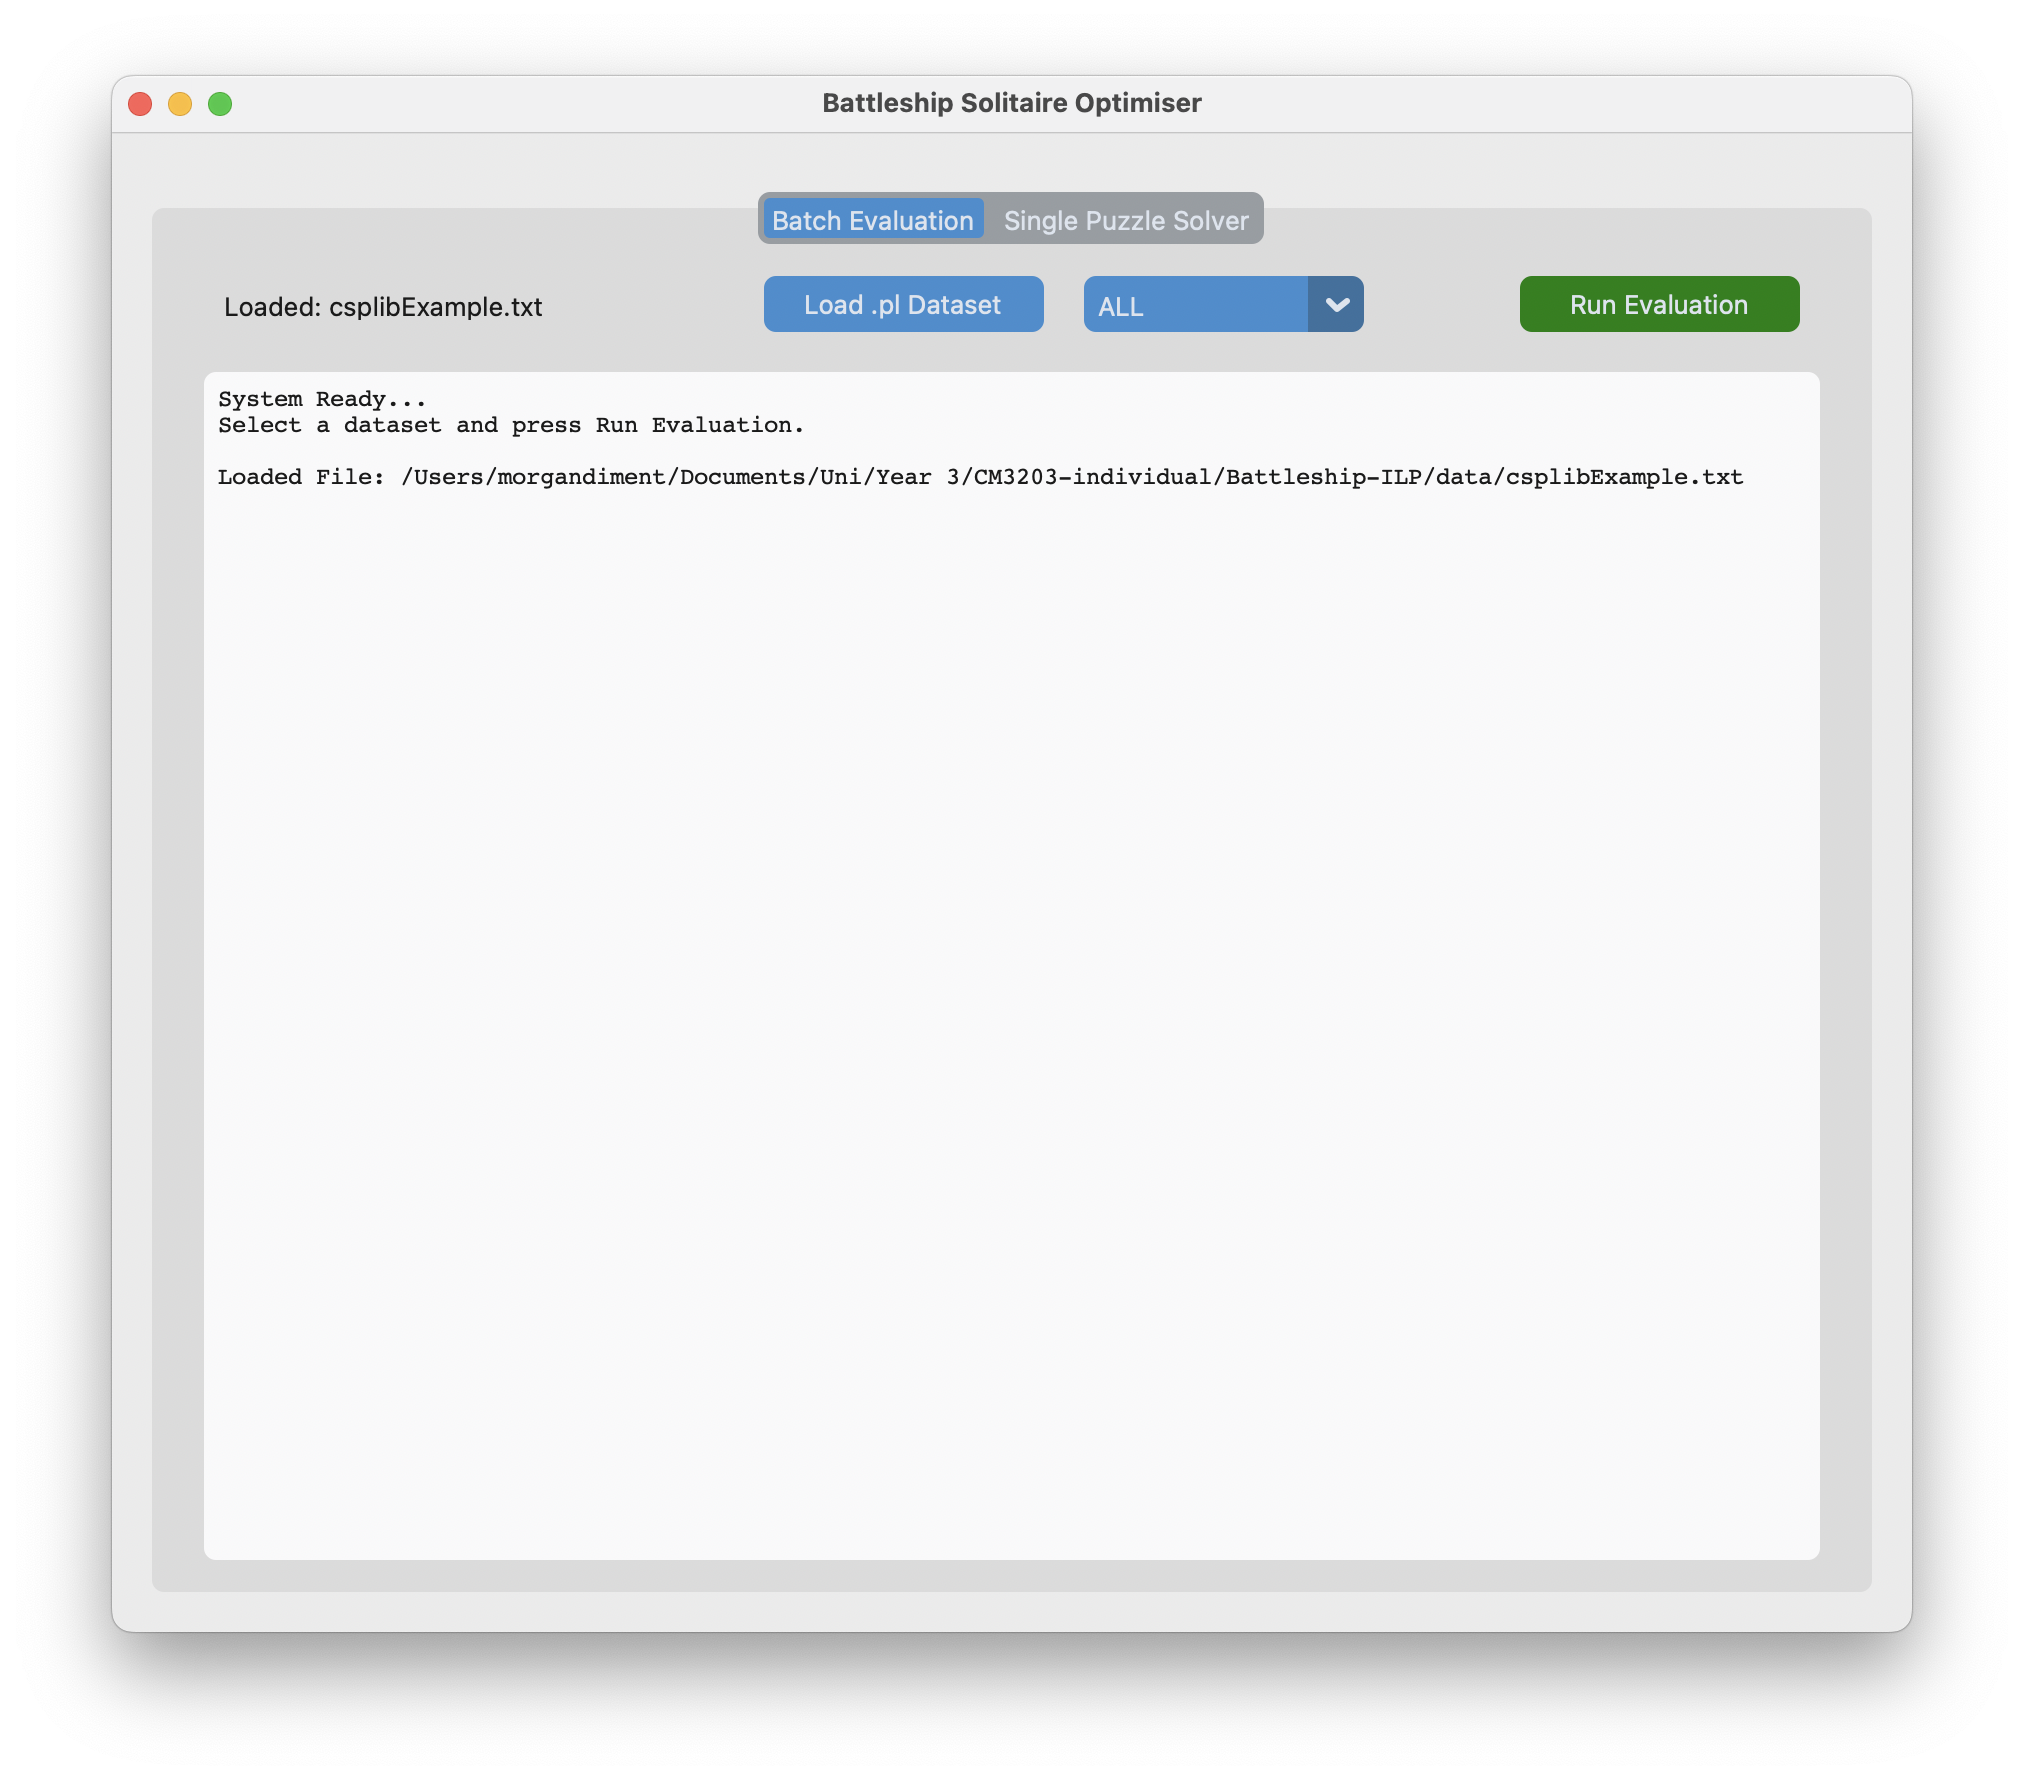
\includegraphics[width=0.95\linewidth]{images/GUI/batch-tab.png}
  \caption{Batch Evaluation tab. The user loads a Prolog dataset file (left), selects which solver(s) to run from the drop-down (centre), and presses ``Run Evaluation''. The console pane streams the per-instance comparison table as the evaluator processes each puzzle, with output marshalled from the background solver thread to the main UI thread through the \texttt{TextboxRedirector} class.}
  \label{fig:gui_batch}
\end{figure}

\begin{figure}[h]
  \centering
  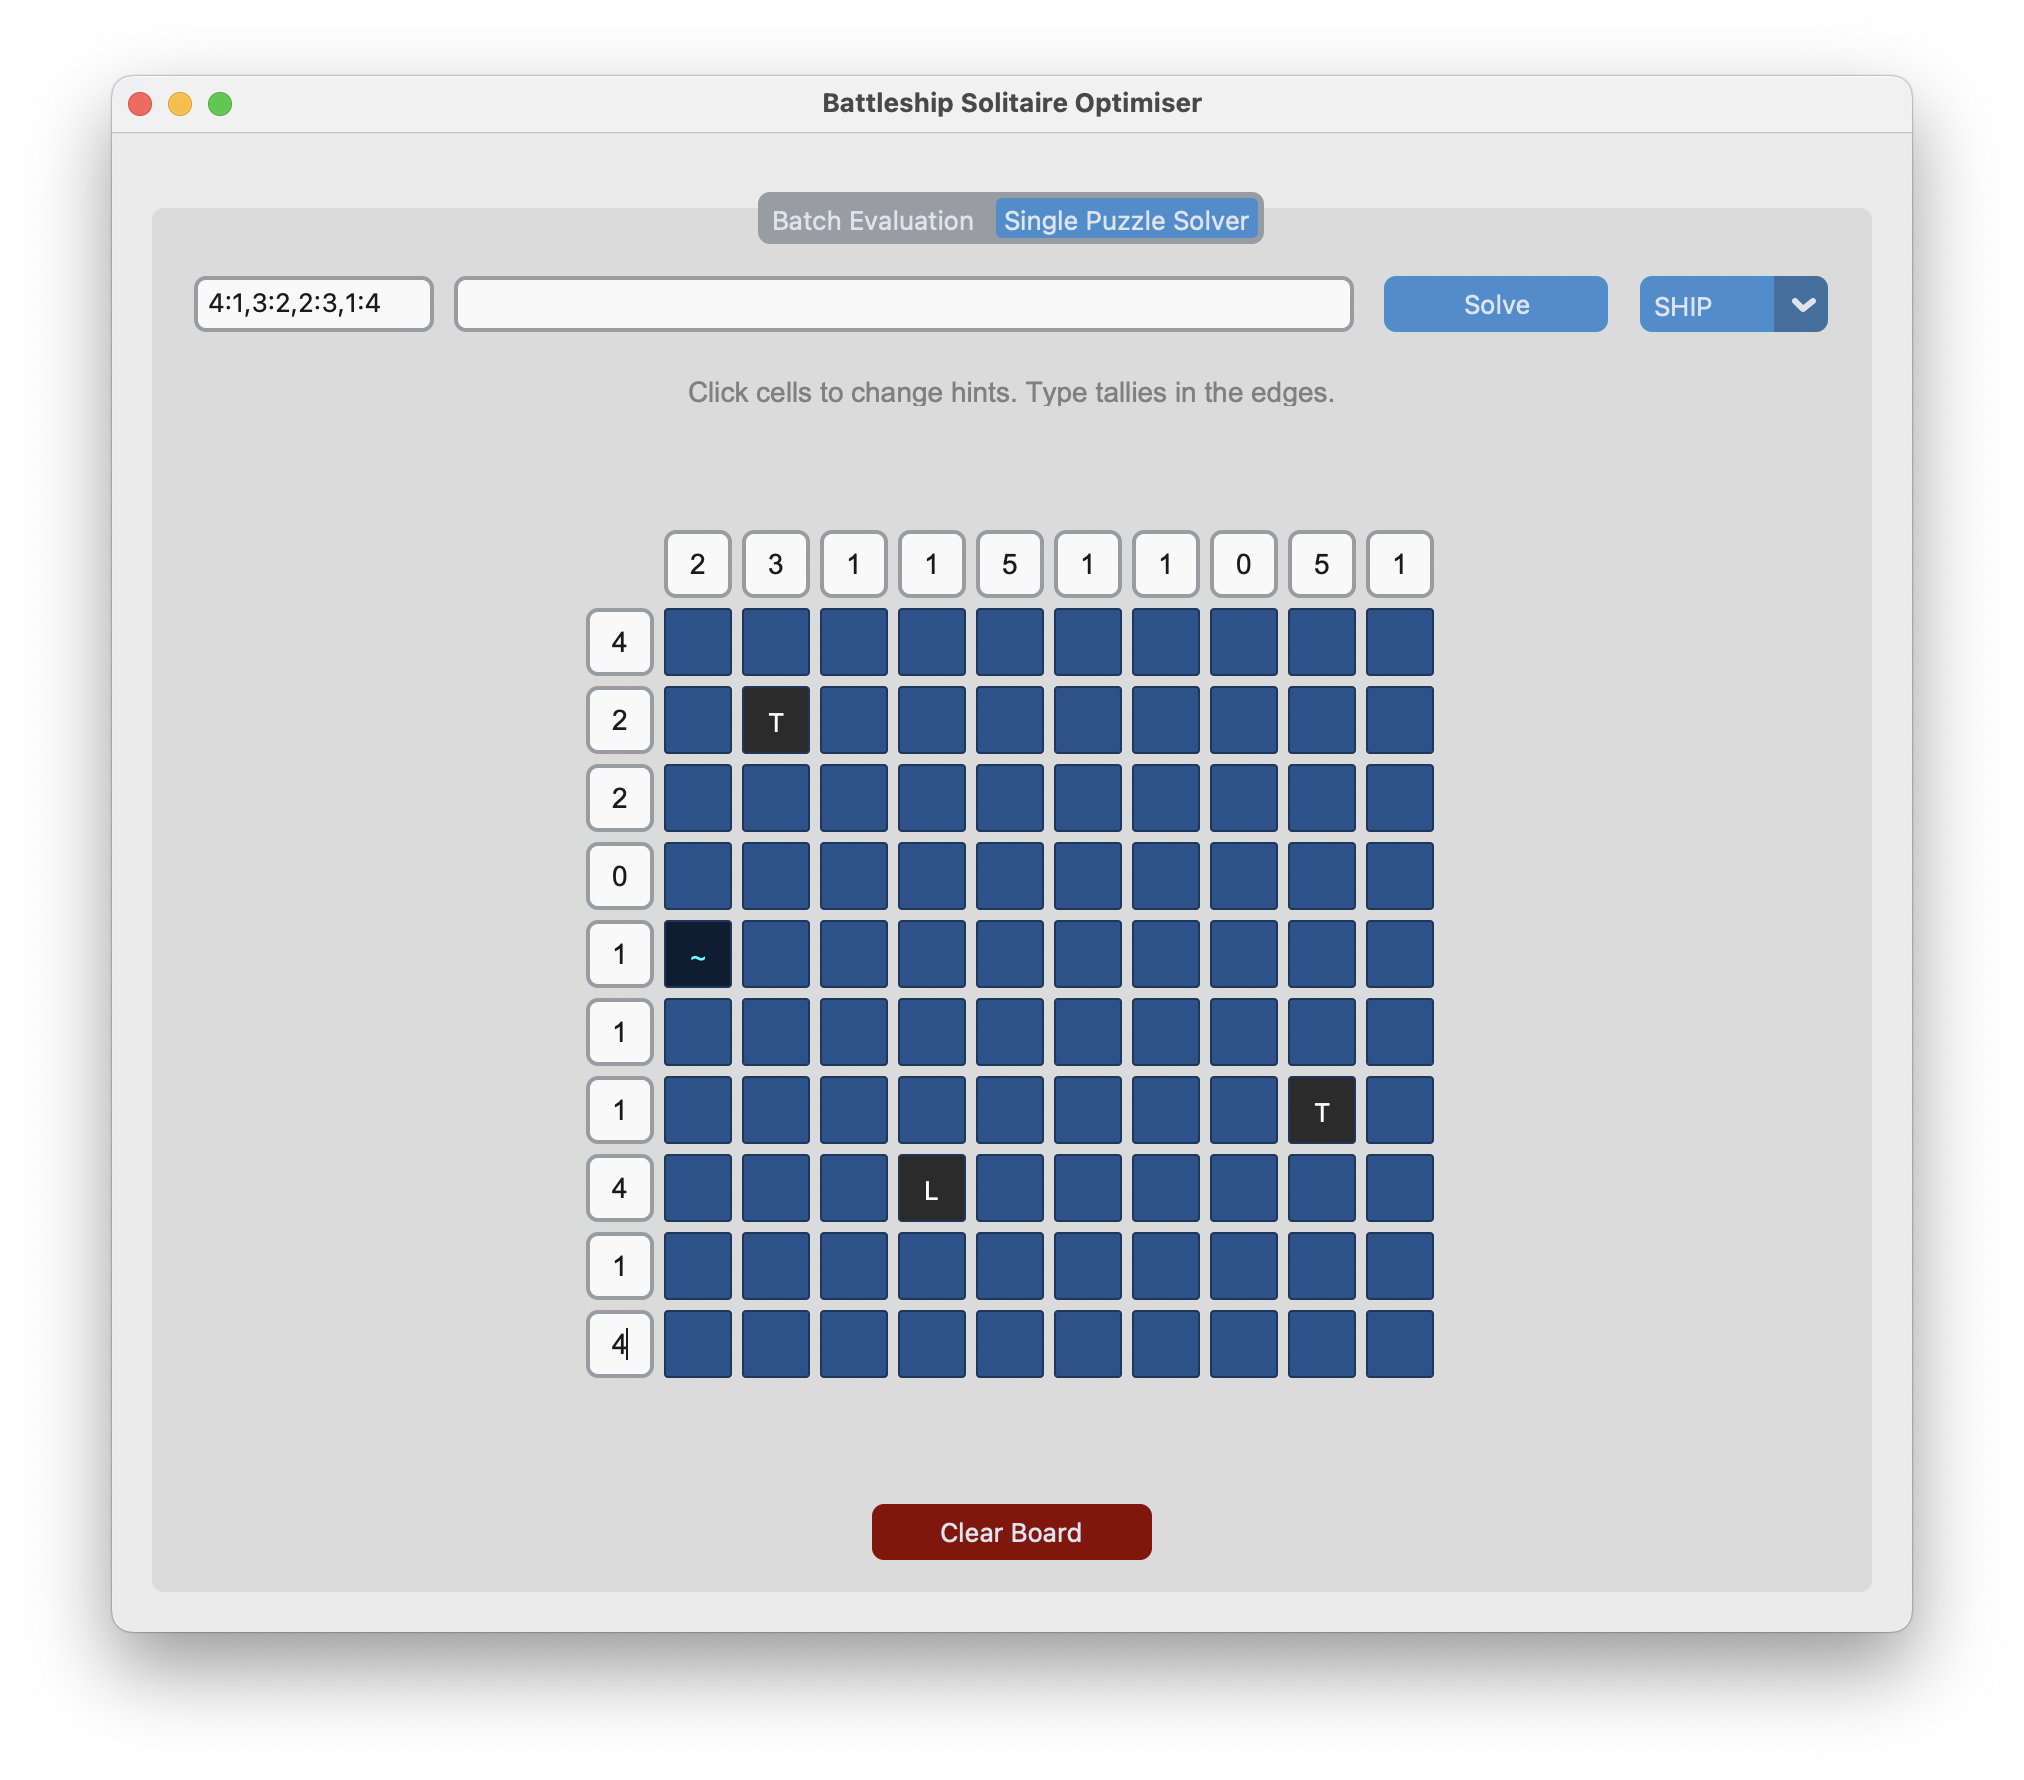
\includegraphics[width=0.95\linewidth]{images/GUI/single-puzzle-unsolved.png}
  \caption{Single Puzzle Solver tab in input mode. The fleet specification, row tallies and column tallies are typed into the bordered input boxes; clicking each grid cell cycles through the seven possible \gls{csplib} states (water, submarine, top, bottom, left, right, middle) for entering hints. The ``Solve'' button dispatches the constructed instance to the chosen solver on a background thread.}
  \label{fig:gui_single_unsolved}
\end{figure}

\begin{figure}[h]
  \centering
  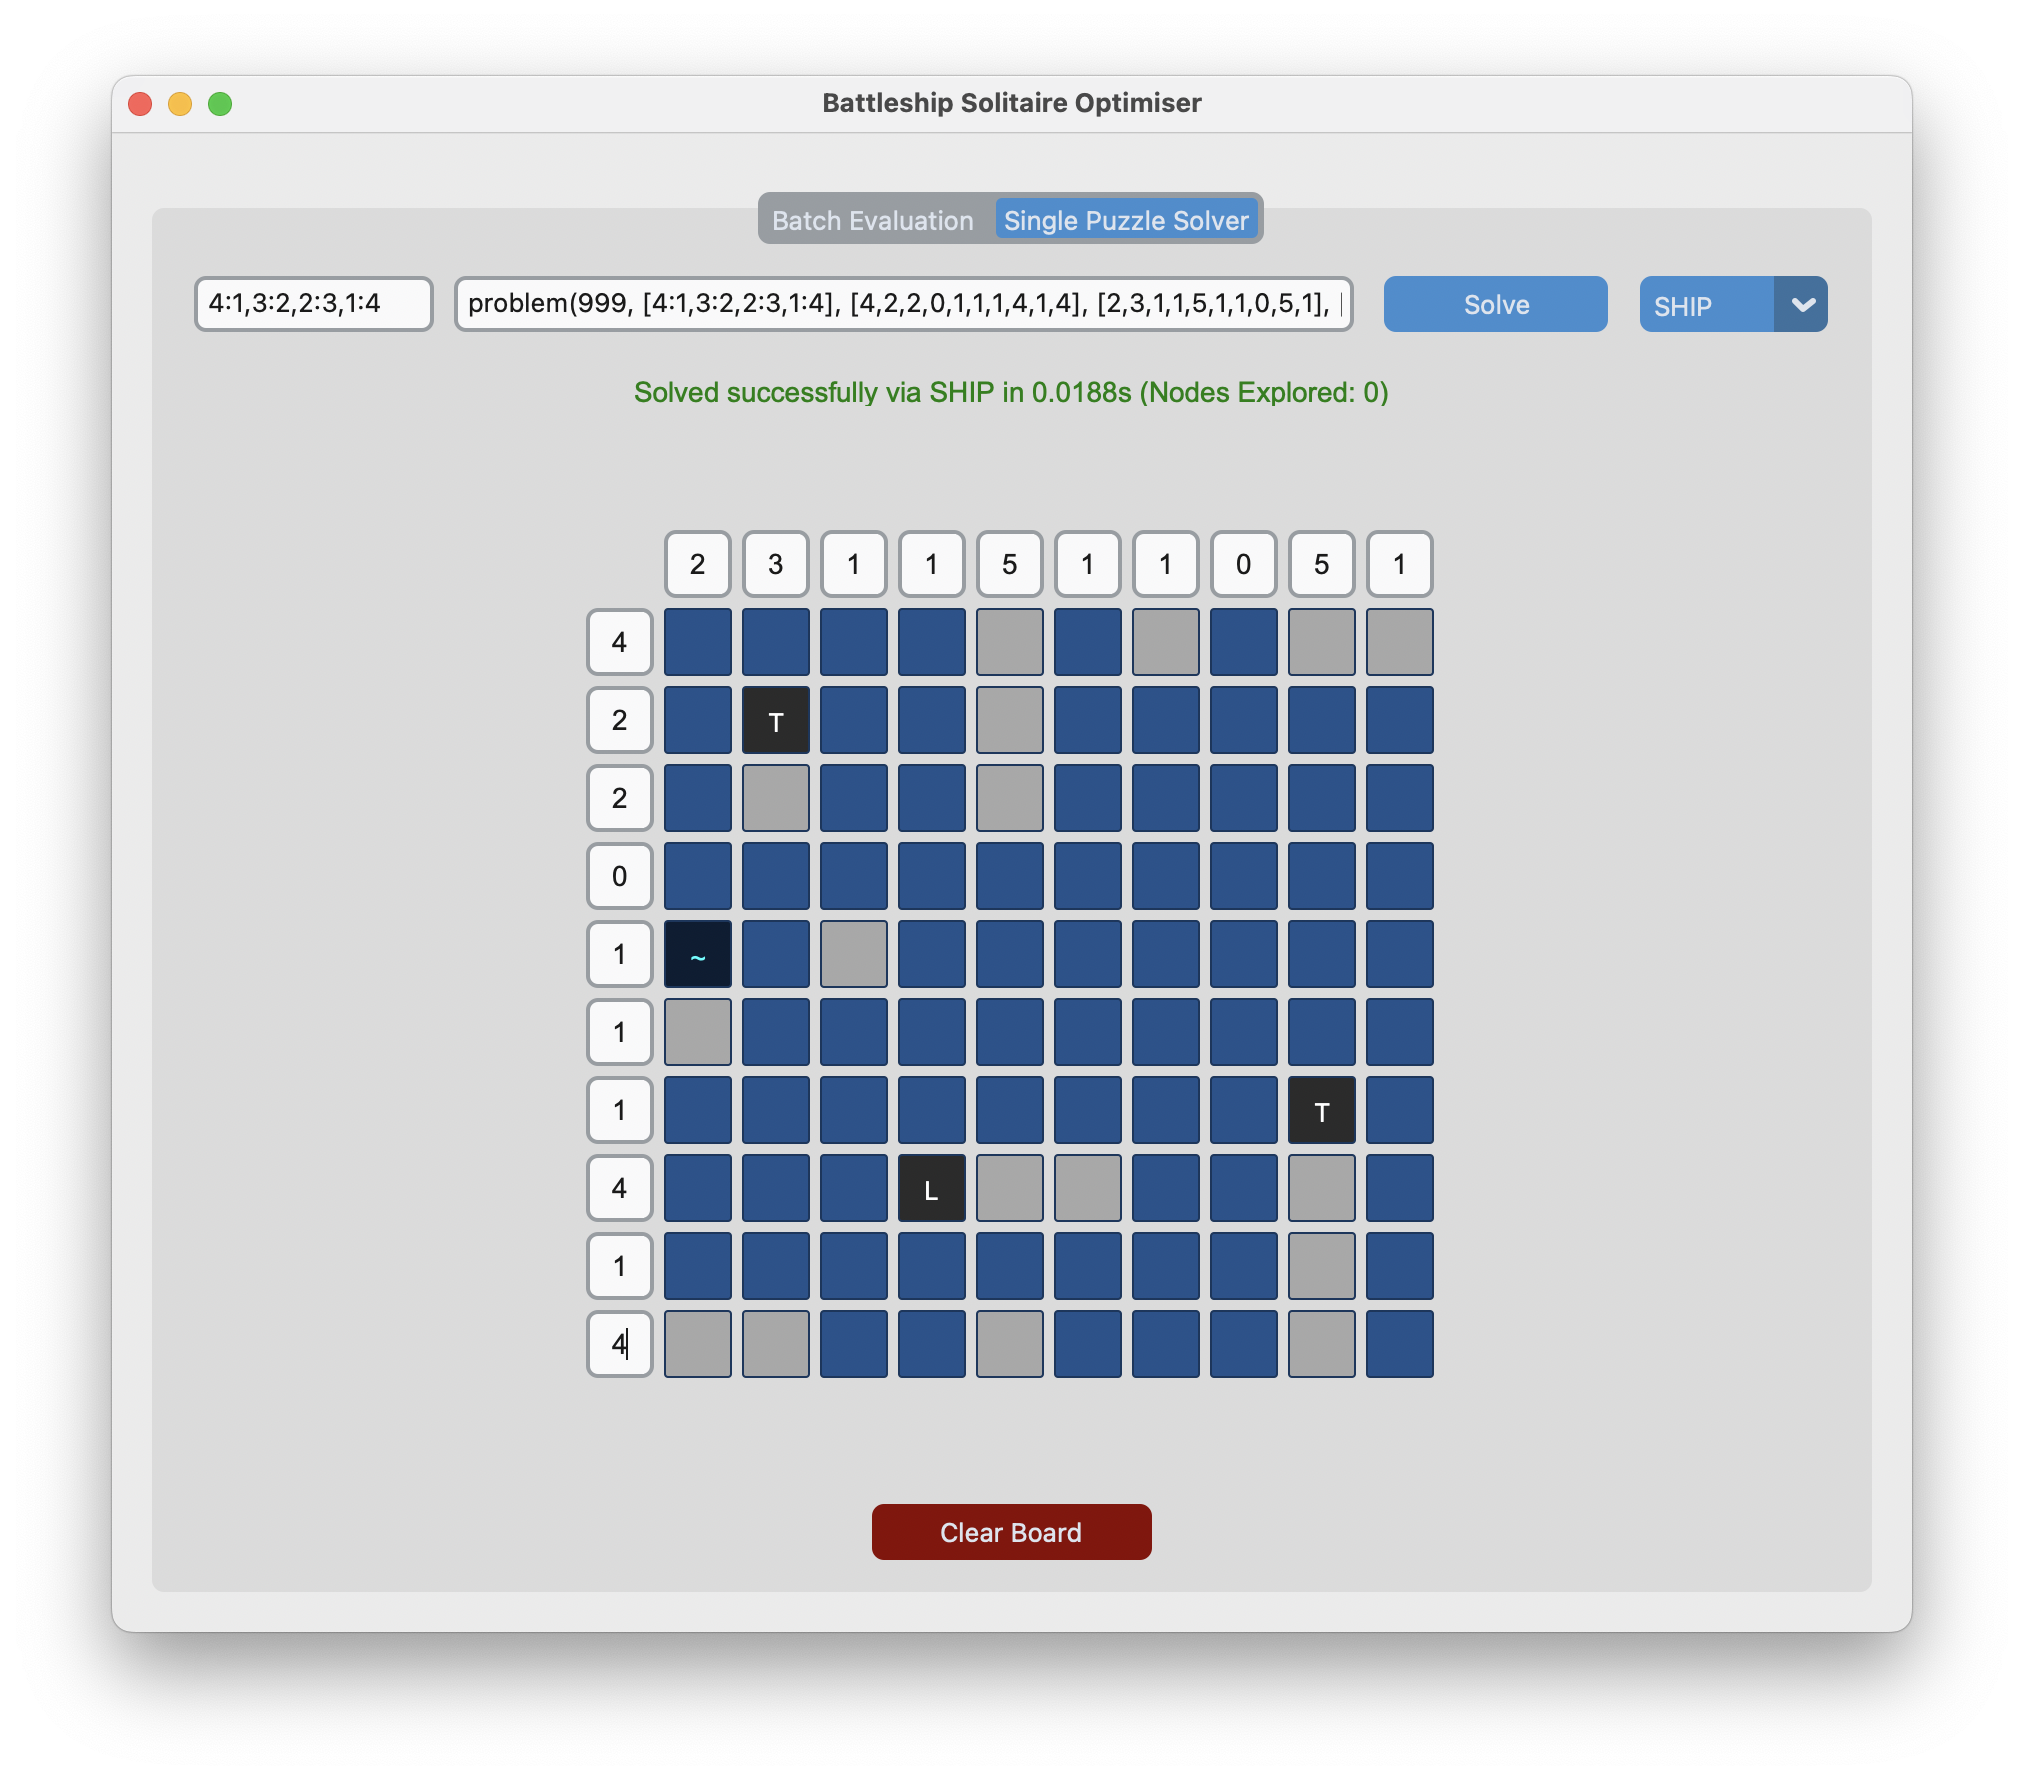
\includegraphics[width=0.95\linewidth]{images/GUI/single-puzzle-solved.png}
  \caption{Single Puzzle Solver tab after solving. The status line reports the wall-clock solve time and the branch-and-bound node count returned by Gurobi. Cells that were not part of the input hint set are repainted in light grey to show the recovered ship placements, and the original hints retain their input colouring.}
  \label{fig:gui_single_solved}
\end{figure}

\chapter{Additional Results}\label{app:results}
% =============================================================================
% Appendix: Supplementary Material
% =============================================================================
% SPDX-FileCopyrightText: 2026 Frank Langbein <frank@langbein.org>
% SPDX-License-Identifier: LPPL-1.3c
%
% Appendices hold supporting material (detailed tables, derivations, survey text,
% user-study materials) so the main narrative stays focused. Complete source
% code is usually submitted separately, not in the report. Use \chapter and
% \section as in main chapters. Replace with your own supplementary material.
% =============================================================================

This appendix contains the per-grid-size and per-difficulty result tables that underlie the figures in Chapter~\ref{ch4}. The numbers are the same evaluation runs that produced Figures~\ref{fig:line_scaling}, \ref{fig:node_complexity}, and~\ref{fig:cuts_comparison}.

\section{Per-grid-size summary on the generated dataset}\label{app:per-size}

For each grid size in the generated dataset (5 sizes $\times$ 8 hint counts $\times$ 5 instances $=$ \num{200} puzzles) the average solve time and the average number of branch-and-bound nodes explored by each model are reported below.

\begin{fullwidthtable}[h]
  \centering
  \caption{Average solve time (seconds) and average branch-and-bound nodes explored, on the 200-instance generated dataset, by grid size and solver. ``Cell (Std)'' denotes the baseline Cell Model; ``Cell (Imp.)'' denotes the Improved variant with all four valid inequalities active.}
  \label{tab:appendix-per-size}
  \begin{tabular}{lcccccc}
    \toprule
    Grid (cells) & Ship time & Cell (Std) time & Cell (Imp.) time & Ship nodes & Cell (Std) nodes & Cell (Imp.) nodes \\
    \midrule
    10$\times$10 (100)  & 0.0103425 & 0.052985 & 0.051805 & 0.53 & 0.57 & 0.57 \\
    15$\times$15 (225)  & 0.01029825 & 1.286185 & 1.30245 & 1.0 & 2.4 & 1.0 \\
    20$\times$20 (400)  & 0.209615 & 2.231215 & 2.7381525 & 1.0 & 1.0 & 1.0 \\
    25$\times$25 (625)  & 0.461325 & 7.0706375 & 9.2635575 & 1.0 & 1.0 & 1.0 \\
    30$\times$30 (900)  & 0.428335 & 11.361165 & 10.03928 & 1.0 & 1.0 & 1.0 \\
    \bottomrule
  \end{tabular}
\end{fullwidthtable}

The numbers in this table are the per-size averages plotted in Figure~\ref{fig:line_scaling} and Figure~\ref{fig:node_complexity}, made explicit so that future work can compare against them quantitatively rather than read them from the chart axes.

\section{CSPLib instance coverage}\label{app:csplib-coverage}

All 303 instances in the standard \gls{csplib} Problem 014 dataset (\verb|data/csplib.pl|) were processed by all three solver variants. Every instance returned a feasible solution under the validator described in Section~\ref{subsec:standard-academic-dataset}. The split by difficulty bracket (defined in Section~\ref{subsec:controlling-scalability-heuristic-diff}) is:

\begin{table}[h]
  \centering
  \caption{Distribution of the 303 \gls{csplib} Problem 014 instances by difficulty bracket. \gls{csplib} contains no Easy instances under the bracketing used in this dissertation; the bracket is included for completeness.}
  \label{tab:appendix-csplib}
  \begin{tabular}{lcc}
    \toprule
    Difficulty & Hint count & Instances \\
    \midrule
    Easy   & $\geq 10$  & 0   \\
    Medium & 4--9       & 22 \\
    Hard   & 0--3       & 281 \\
    \midrule
    \multicolumn{2}{r}{Total:} & 303 \\
    \bottomrule
  \end{tabular}
\end{table}

Of these instances, all were solved successfully (no timeouts, no infeasibility errors) by every solver variant, providing end-to-end evidence that the parser, the data ingestion layer, and both \gls{ilp} formulations operate correctly on standard published puzzles.



% Bibliography (always last): \bib{bibfile} uses natbib (numeric or harvard per class option)
% and inserts the License chapter if \license was set.
\bib{bibliography}

\end{document}
